\section{Introduction}\label{sec:introduction}
\frame{\tableofcontents[currentsection]}

%-------------------------------------------------
\subsection{Domain Context}\label{subsec:domain-context}
\begin{frame}
    \frametitle{Domain Context}
    The concept of \textbf{Micro City} was born observing contexts in which \textit{self-awareness} and \textit{situatedness} might help improve people's experience.

    \bigskip

    We believe that in these contexts wearable devices (and applications running on them) can have a great impact on how people interact with the environment.

\end{frame}
%------------------------------------------------

\subsection{What is a Micro City?}\label{subsec:what-is-a-micro-city?}
\begin{frame}
    \frametitle{What is a Micro City?}
    A \textit{Micro City} is an area with:
    \begin{itemize}
        \item bounded temporal and spatial extension;
        \item various activities in the form of services or events;
        \item people (\textit{guests}) that are interested in these activities and populate the \textit{Micro City} itself because of them;
    \end{itemize}

    \bigskip

    Thus, some examples of \textit{Micro Cities} could be shopping centers, fairs, \textit{amusement parks}, city centers, etc.

\end{frame}
%------------------------------------------------

\subsection{Recommendations}\label{subsec:recommendations}
\begin{frame}
    \frametitle{Recommendations}
    In this context, the introduction of a \textbf{situated recommendation system} could proactively provide recommendations to the guests that, if willing to follow them, would receive rewards.

    \bigskip

    The recommendations could be generated thanks to various policies and the rewards could vary depending on the context of the \textit{Micro City} itself (discounts, cashback, simple reduction of waiting time, etc.)
\end{frame}
%------------------------------------------------

\begin{frame}
    \frametitle{Rewards}
    \begin{columns}
        \begin{column}{0.5\textwidth}
            \begin{addmargin}[0.6em]{2em}
                The following diagram shows the process of obtaining a reward when receiving a recommendation.
            \end{addmargin}
        \end{column}
        \begin{column}{0.5\textwidth}
            \begin{center}
                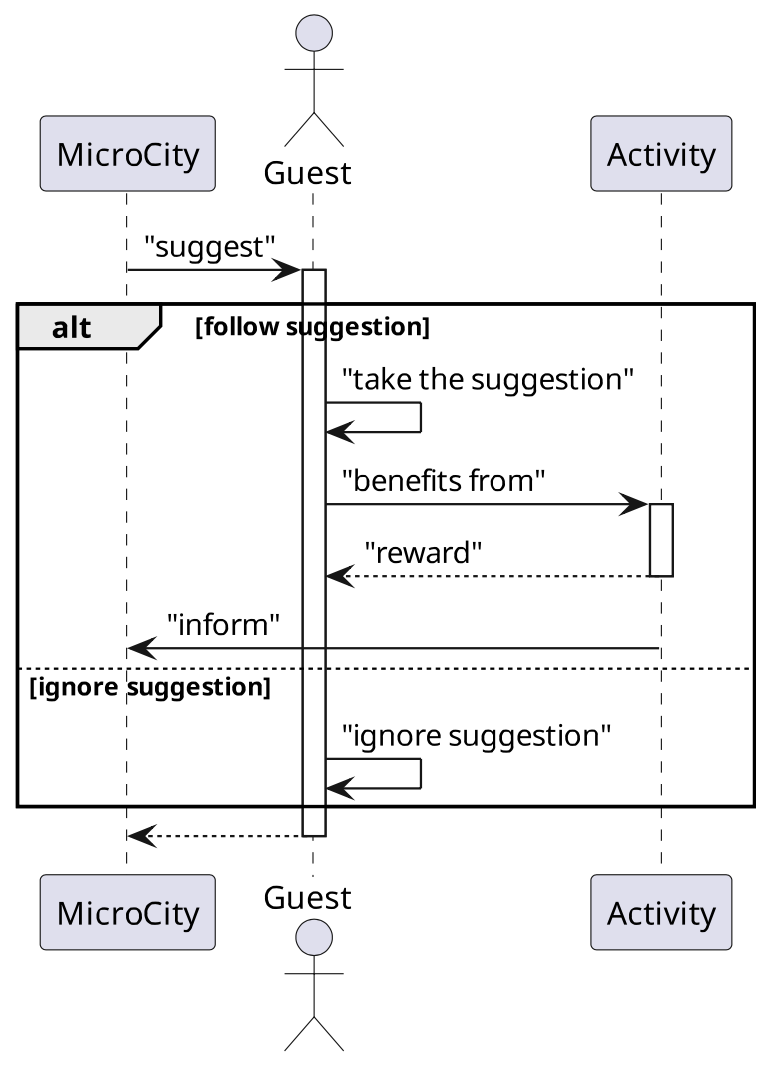
\includegraphics[width=0.9\textwidth]{../img/rewards}
                \label{fig:rewards}
            \end{center}
        \end{column}
    \end{columns}
\end{frame}

